The submitted code is split into two libraries, each kept in a separate repository.
The first library, called \texttt{PerpleX-cpp}, contains the C++ wrapper code for Perple\_X and consists of both Fortran and C++ code.
The second, called \texttt{PerpleX-ASPECT}, predictably contains the plugin code that implements the wrapper inside of ASPECT and is written entirely in C++.
A diagram displaying the relations between the repositories as well as Perple\_X and ASPECT are shown in Figure~\ref{fig:dataflow}.
Alongside the source code, a wiki is provided giving useful information about things such as setting up a development environment on the Hamilton supercomputer, viewing the results in Paraview, and using Docker.

The justification for splitting the code into two repositories is twofold.
Firstly it ensures that the Perple\_X wrapper code is entirely general and the library can be used outside of ASPECT.
Secondly, it enforces a separation between the ASPECT code and the wrapper.
This is potentially valuable were the plugin code to be integrated upstream into the main ASPECT repository.

The code for both libraries is compiled using CMake.
CMake is a cross-platform build tool that can generate native makefiles and handle testing through CTest.
It was a requirement for the ASPECT plugin code as the ASPECT developers provide a CMake script that links the code to ASPECT and the underlying deal.II library.
However, it was very helpful to also compile the plugin code using CMake because integrating libraries is straightforward.

Regarding the code licensing, both Perple\_X and ASPECT are licensed under the GNU Public License (GPL) version 2.
In order for the submitted code to be compliant with these licences it has been licenced using the more modern GPL version 3.

\begin{figure}[ht]
    \centering
    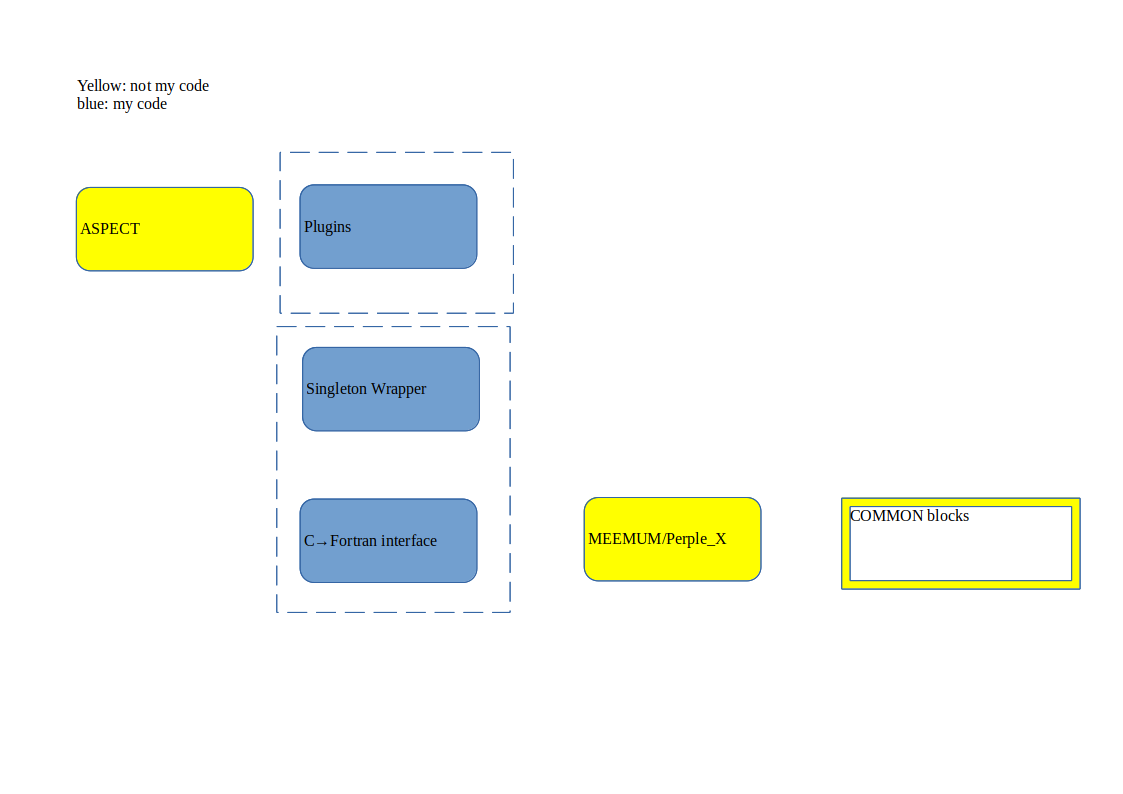
\includegraphics[width=\textwidth]{figures/dataflow.png}
    \caption{Diagram displaying the flow of data through the program. The blue blocks represent the new code and the yellow blocks represent the reused code.}
    \label{fig:dataflow}
\end{figure}

\subsection{Perple\_X C++ wrapper code}

The Perple\_X wrapper library presents two main functions to the user: one to initialise Perple\_X and the other to perform the MEEMUM computation and return the result.
It aims to abstract away to the greatest extent possible the complexities of dealing with the Perple\_X codebase.
For example, the only argument necessary to initialise the wrapper code is the path to the Perple\_X problem file and the only arguments needed to perform a subsequent calculation are the pressure, temperature and composition (which is just an array).

\subsubsection{Original Perple\_X source code}

Starting from the Perple\_X code and working up to the wrapper (see Figure~\ref{fig:dataflow}), the first component of the library is the Perple\_X source itself.
The decision was made to directly include the source code inside the repository rather than either encouraging the user to install Perple\_X themselves or retrieving via a URL.
The principle reason for this is reliability, Perple\_X receives frequent breaking updates and there is no easy way to access old versions so in order to ensure that the code remains in a usable state the source code is stored inside the repository.
The version used in the repository at the time of writing is 6.9.0.
Despite adding the code to the repository and tracking changes, the code has not been changed from the original Perple\_X code at all.
This is to try and minimise the amount of issues that will occur if at any point the Perple\_X version is ever upgraded.
Additionally the codebase is actually relatively small so inclusion does not create any significant overhead.
MEEMUM only depends on 8 (at the time of writing) source files and compilation occurs in well under a minute.

When Perple\_X is downloaded it comes with many files that compile to different executables other than MEEMUM as well as lots of thermodynamic database files and various README's.
To avoid confusion, only the necessary source files are included inside the repository.

\subsubsection{Fortran-to-C++ interface}

The basic concept of integrating Fortran code into C++ is very simple, all that is required is a C++ header file declaring the needed Fortran functions and variables using the correct symbols (e.g. the function \texttt{foo()} is normally represented with the symbol \texttt{foo\_} by the linker) and then the codes can be linked during compilation.
However, actually implementing this is far from straightforward: many of the data types are incompatible, array indexing starts from zero (C++) or one (Fortran) and arrays themselves are alternately row-major order (C++) and column-major order (Fortran).

This problem is compounded in Perple\_X by the sheer number of global variables, both constant PARAMETER's and COMMON blocks that are used by the program.
The source code contains a 400 line file called \texttt{perplex\_parameters.h} that contains the program parameters as well as lots of frequently used COMMON blocks.
If one were to write a C++ wrapper then this file would need to be converted into a C++ header as well as any MEEMUM specific code.

This was the approach taken previously by ???. A Python script was written that `compiled' the Fortran parameter file into a C++ header permitting linking.

However, this approach has a number of serious drawbacks: (a) whenever Perple\_X is upgraded this script must be re-run (b) the process is complex and hard to debug in case errors occur (c) the resulting header file is hard to read.

To solve these issues, an additional Fortran file was included in the codebase to `sanitise' the interface.
It provides a small number of property getters and setters as well as a largely verbatim copy of the MEEMUM subroutine, only altered to eliminate any calls for user input and split into initialise (called once) and compute (called many times) sections.
Arguments are passed by value (C-like) and only single values are passed (excluding strings), avoiding any complexities involved with arrays.

An additional advantage of this approach is readability.
Being written in Fortran 77, Perple\_X has a 6 character limit on its variable names which can make it very hard to follow what the variables and functions do.
The new interface code was not so restricted allowing for much more verbose function names.

\subsubsection{Singleton wrapper}

Although the basic interface described above is a significant improvement on previous approaches, it is still fairly limited.
Only basic data types are accepted and its use requires interacting with global variables, something that is considered poor software development practice.

Our solution to both these problems is the creation of a \texttt{Wrapper} class.
The class presents initialise and compute methods to the user and hides the details of interfacing with the Fortran at all.
It additionally permits the use of more complex data types, such as \texttt{std::vector} and \texttt{std::string} that are in common use in ASPECT.
An object-oriented solution was chosen because Perple\_X consists of both functions and data, making it a good idea to group them together into a class.

The class also implements the \textit{singleton pattern}, that is, only a single instance of the class may ever exist at the same time.
This approach was taken in order to prevent concurrent accesses to the Perple\_X data structures that are global.

During the project, it was noticed that many computations were being done with either identical or almost identical inputs. 
It therefore made sense to store the most frequently used results and use them if the inputs are sufficiently similar.
A cache was implemented using a least recently used (LRU) eviction policy.
A flowchart detailing the decision process for a LRU cache is shown in Figure~\ref{fig:cache_flowchart}.

\begin{figure}[ht]
    \centering
    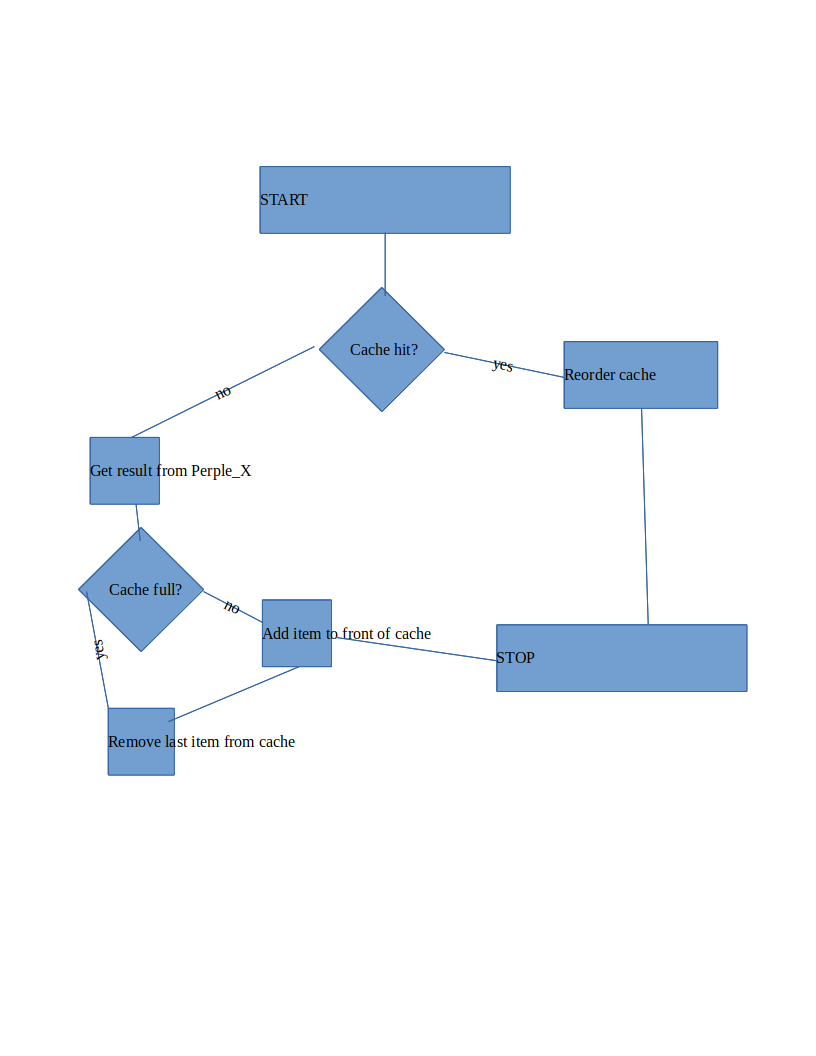
\includegraphics[width=\columnwidth]{./figures/cache_flowchart.png}
    \caption{Flowchart showing the decision process for the least recently used (LRU) cache used by the \texttt{Wrapper} class.}
    \label{fig:cache_flowchart}
\end{figure}

\subsubsection{Testing}

The library is tested using the Google C++ unit testing framework Google Test.
For the Fortran-to-C++ interface and singleton wrapper class, the tests consist largely of a direct comparison between the results of the function calls and previously collected MEEMUM output for a quick-to-run sample data set.

\subsubsection{Parallelism}

Perple\_X is not designed for parallel execution and as such the library is not thread-safe. 
However, there are only several methods that are exposed to the user so it would be straightforward to add locks to these methods making them thread-safe.
In contrast, the code is entirely suitable for parallel use in a distributed memory environment (i.e. MPI) because the global state is still local to each processor.
MPI is the primary parallelisation method used within ASPECT and so thread-safety was not considered a necessary feature of the library.

\subsection{ASPECT plugins}

The Perple\_X wrapper code was integrated into ASPECT using ASPECT's powerful plugin system.
Plugins are compiled into shared libraries with CMake.
These are libraries that are linked to at runtime, rather than compile time which is for static libraries.
Although care must be taken to use the same compiler for the plugin as for the main ASPECT binary this approach has significant advantage that it does not require recompilation of the main ASPECT binary every time.

The decision was taken to implement the code using the plugin system rather than forking the main ASPECT repository for the following reasons: 
(a) updating ASPECT does not require either rebasing or merging the git repositories 
(b) not having the new code mixed in with the original code makes things clearer 
(c) the code is rather specialist and may not ultimately be added to the ASPECT codebase.

The plugins expose to the user a set of options that may be included in the parameter file that is submitted to ASPECT.
Given the small number of source files that are written, no automatic method of generating the documentation has been written and we recommend reading the source code for parameter details.

Some example parameter files are included in the \texttt{cookbooks} component of the repository.
These provide examples of the various functionality of the plugins.

Regarding the actual plugins that were written, two different approaches were taken to track the Perple\_X composition in ASPECT: compositional fields (via a material model) and particles.
The details of their implementation will be discussed next.

\subsubsection{Particle plugin}

As discussed in Section~\ref{sec:introduction}, the basic idea of particles in a geodynamical simulation is that they are point objects passively advected around the medium with the velocity field.
At set timesteps they are then `evaluated' using the state of the different fields present at their current position.
In this work, a \textit{particle property} plugin was written that returns phase information from Perple\_X using the pressure, temperature, and, at least initially, bulk composition from the specified Perple\_X problem file.

The precise information that the plugin reports depends upon the options specified in the parameter file.
At present the possible properties that may be reported by the plugin for each endmember phase are the: composition, molar amount (in moles), molar fraction, volume fraction, and weight fraction.
This list would be straightforward to extend to any of the properties reported as output from MEEMUM and serves mainly as a proof-of-concept.

One particularly noteworthy set of options permitted by the plugin are \texttt{Extract melt} and \texttt{Melt extraction threshold}.
These permit an investigation of fractional melting of the material (see Section~\ref{sec:introduction} for a discussion of this).
If \texttt{Extract melt} is set to \texttt{true} then the particle will automatically report on the amount of moles of the melt that is extracted and on its composition.
Fractional properties (e.g. weight fraction) of the extracted melt are not tracked due to being non-physical.

\subsubsection{Material model plugin}

The ability to easily control the number of particles and evaluation rate is extremely useful for investigations with MEEMUM because each evaluation can take a considerable amount of time to complete.
The approach additionally permits the use of any material model.

However, it was found that the particle-based approach was incompatible with a study of two-phase flow.
This is because two-phase flow requires that the composition of the melt be advected separately to the composition of the residue.
In ASPECT particles can be set to \textit{either} advect with the melt field or with the solid material, but not both.
The underlying implementation of particles in ASPECT does not permit them to be differentiated into different classes.
Therefore there would be no way to use particles in a study of two-phase flow without a radical change to the ASPECT source code.

In this work we avoided this problem by pivoting to a compositional field-based approach and implementing a material model plugin.
In the simulation there are compositional fields for each component in the composition for both the melt and residue and these fields advect with either the solid or melt.

An unfortunate downside to this approach is that the parameter files become significantly more complex as the compositional fields must be specified by name and must correspond exactly to the compounds specified in the Perple\_X problem file.

The first material model plugin to be implemented used the ASPECT model \texttt{melt simple} as the underlying base model with some logic for calling MEEMUM and updating the relevant compositional fields on top.
This simplified development and ensured that any results from the simulation would be physically reasonable but had a significant downside in that the actual fraction of melt that was reported came from a simple parametrisation rather than from the composition-aware MEEMUM computation.
This not only makes the results less accurate, but it causes inconsistencies in the results such as when, for example, the ASPECT function reports the presence of melt but Perple\_X does not. 
In this situation the melt is reported as having no composition.

In an effort to mitigate the amount of disparity between the two models, the temperature being passed to Perple\_X is increased by $200 \mathrm{K}$.
This obviously impacts upon how reasonable the results can be considered to be.

To try and fix these issues, a material model that calculates the melt fraction using Perple\_X was also created.
However, the code experienced serious convergence issues and we ran out of time.
The code (\texttt{perplex\_melt.cc}) is included in the repository should anyone wish to get it working in future.

\subsubsection{Additional plugins}

In addition to the plugins discussed above, \textit{postprocessor} and \textit{initial composition} plugins were also written.
The postprocessor plugin is called \texttt{perplex cache statistics} and it permits analysis of the cache in the Perple\_X wrapper.
The initial composition plugin is called \texttt{perplex composition} and it makes sure that the compositional fields representing the melt and residue compositions (for two-phase flow) are initialised correctly.

\subsubsection{Testing}

Unit testing is difficult to do in ASPECT, as evidenced by the fact that very few actually exist in the main repository, due to the fact that plugins are tightly integrated with the rest of the simulation.
Most plugins inherit from the \texttt{SimulatorAccess} class in order to access information from the rest of the simulation such as time step number or to interact with other plugins.
Such complex interactions make typical unit testing of single pieces of functionality practically impossible.

Instead of using unit tests, ASPECT relies upon \textit{benchmarks} for evidence of its accuracy.
These involve running simulations with a known answer, for example the temperature change over a phase transition, and verifying that the ASPECT code converges to the correct answer.
The decision was made to not include any benchmarks with the code because they require detailed domain-specific knowledge and we were running out of time.

The other form of tests used in ASPECT simply compares the output of a simulation with a previous run to ensure that the results are unchanged.
Tests of this nature were not included in the code because the CMake script necessary to perform such a test is complex and we were limited by time.
